
%%%%%%%%%%%%%%%%%%%%%%%%%%%%%%%%%%%%%%%%%%%%%%%%%%%%%%%%%%%%%%%%%%%%%%%%%%%%%
%
%  System        : 
%  Module        : 
%  Object Name   : $RCSfile$
%  Revision      : $Revision$
%  Date          : $Date$
%  Author        : $Author$
%  Created By    : Jim Finnis
%  Created       : Mon Oct 4 09:50:39 2010
%  Last Modified : <160420.1323>
%
%  Description 
%
%  Notes
%
%  History
% 
%%%%%%%%%%%%%%%%%%%%%%%%%%%%%%%%%%%%%%%%%%%%%%%%%%%%%%%%%%%%%%%%%%%%%%%%%%%%%
%
% Copyright (c) 2010 Jim Finnis.
% 
% All Rights Reserved.
% 
% This  document  may  not, in  whole  or in  part, be  copied,  photocopied,
% reproduced,  translated,  or  reduced to any  electronic  medium or machine
% readable form without prior written consent from Jim Finnis.
%
%%%%%%%%%%%%%%%%%%%%%%%%%%%%%%%%%%%%%%%%%%%%%%%%%%%%%%%%%%%%%%%%%%%%%%%%%%%%%

\documentclass[a4paper]{article}
\usepackage{wrapfig}
\usepackage[pdftex]{graphicx}
%\usepackage[version=3]{mhchem}
\usepackage{fancyvrb}
\usepackage{multirow}
\usepackage{url}
\usepackage{amssymb}
\usepackage{enumitem}

\usepackage[hmargin=2.5cm,vmargin=3.5cm]{geometry}
\usepackage{multicol}
% In math mode, put a word into text inside anglebrackets. Used for BNF, sometimes.
\newcommand{\angb}[1]{\text{$<$\\#1$>$}}

% so we can do 3\e{4} to do 3x10^4
%\providecommand{\e}[1]{\ensuremath{\times 10^{#1}}}
\providecommand{\e}[1]{\emph{#1}}

\newenvironment{prettycode}
{\begin{quote}\ttfamily\small}
{\end{quote}}


\DefineVerbatimEnvironment{v}{Verbatim}{
    %numbers=left,numbersep=5pt,
    %frame=lines,framerule=0.5mm,
    fontsize=\small,xleftmargin=15pt}
\DefineVerbatimEnvironment{vv}{Verbatim}{
    %numbers=left,numbersep=5pt,
    %frame=lines,framerule=0.5mm,
    fontsize=\small,xleftmargin=15pt}
\DefineVerbatimEnvironment{v2}{Verbatim}{
    %numbers=left,numbersep=5pt,
    %frame=lines,framerule=0.5mm,
    fontsize=\scriptsize,xleftmargin=0pt}
\DefineVerbatimEnvironment{v3}{Verbatim}{
    %numbers=left,numbersep=5pt,
    %frame=lines,framerule=0.5mm,
    fontsize=\tiny,xleftmargin=0pt}
\DefineVerbatimEnvironment{bv2}{BVerbatim}{
    %numbers=left,numbersep=5pt,
    %frame=lines,framerule=0.5mm,
    fontsize=\scriptsize,xleftmargin=0pt}
\DefineVerbatimEnvironment{bv}{BVerbatim}{
    %numbers=left,numbersep=5pt,
    %frame=lines,framerule=0.5mm,
    fontsize=\scriptsize,xleftmargin=0pt}
\DefineVerbatimEnvironment{bvc}{BVerbatim}{
    %numbers=left,numbersep=5pt,
    %frame=lines,framerule=0.5mm
    commandchars=+\[\],
    fontsize=\scriptsize,xleftmargin=0pt}

\setcounter{secnumdepth}{5}
\setcounter{tocdepth}{5}

\title{Monitor program documentation}
\date{2013}
\author{James Finnis, jaf18@aber.ac.uk}

\begin{document}
\maketitle
\newpage
\tableofcontents

\newcommand{\isqc}{$\mathrm{I}^2\mathrm{C}$}

\newcommand{\todo}[1]{
    \begin{center}
    \fbox{\parbox{4in}{\textbf{To Do}\vspace*{1em} \\#1}}
    \end{center}}
    
% level 2 lists are normally indicated by dashes - I'm changing this
% because it looks too much like a minus sign.
\renewcommand{\labelitemii}{$\circ$}

\section{Introduction}
The \textbf{monitor} program is a Qt-based program for monitoring
and controlling remote systems (typically robots) using key/value pairs
sent as text over UDP channels. The program takes a configuration
file describing the variables to be monitored and UI widgets viewing
those variables (or expressions based on them). Certain widgets 
can also send data to the remote.

\subsection{Requirements}
\begin{itemize}
\item Qt version 5 (change from previous versions, which were Qt4, in
order to have Marble still working without having to compile it)
\item The Marble widget for displaying maps
\item Compiled under Ubuntu -- should work, but untested on anything else
\end{itemize}

\subsection{Compilation}
\begin{itemize}
\item Install Qt5
\item Install Marble (see \url{https://marble.kde.org/install.php}) --
under Ubuntu this entails installing the \texttt{marble} and \texttt{libmarble-dev}
packages
\item From the main directory, run \texttt{qmake} to build the makefile, then run \texttt{make}
\item Once built, test by running \texttt{./monitor -f exampleconfig}
\end{itemize}

\subsection{Receiving data}
Typically, the remote system sends lines of data which looks like this:
\begin{v}
time=13.0 x=1 y=2 someval=100
time=13.2 x=0
time=13.5 x=1 y=2
\end{v}
That is, space-separated key/value pairs containing a mandatory
timestamp. Values are all numerical (floating point).

\subsection{Sending data}
Some monitor widgets can also send data to the remote. This data
is also in space-separated key-value pairs.

\subsection{Running}
To run the monitor, use the command
\begin{v}
./monitor -f configfile
\end{v}
where \texttt{configfile} is the name of a valid configuration file.

\section{Blocks}
A file consist of blocks, which are either:
\begin{itemize}
\item variable blocks, describing the variables expected from the UDP client;
\item window definitions, describing the windows and the frames and widgets within them;
\item audio warning definitions;
\item waypoint extra data definitions;
\item configuration options.
\end{itemize}

\begin{v}
file        ::= { block }

block       ::= varblock
            |   window
            |   audio
            |   waypointdef
            |   configoption
\end{v}

\subsection{Configuration options}
These are defined at the top level:
\begin{itemize}
\item \textbf{validtime} : if a data buffer has not received data for this long, the data in the buffer is 
considered to be invalid. This is useful when there is a reasonably good connection and a long wait between updates
is a symptom of a fault. It is set by default to a very long interval (about two years.)
\item \textbf{port} : this is the port to which the system should listen for UDP packets --- by default 13231, although
it can be set with the \verb+-p+ option on the command line, which will override any value set in the configuration file.
\item \textbf{sendport} : this is the port number for UDP control packets, by default 33333. 
\item \textbf{sendaddr} : this is the address to which control packets are sent. Only set this if you want to override the default
setting, which is to send to the address from which the first telemetry packet comes.
\item \textbf{sendinterval} : the interval between sends of UDP packets for \emph{always send} widgets, by default 2 seconds.
\item \textbf{updateinterval} : the time between ticks at which all graphics are updated, by default 2 seconds.
\end{itemize}
\begin{v}
configoption::= 'port' int
            |   'sendport' int
            |   'sendaddr' string
            |   'validtime' float
            |   'sendinterval' float
            |   'updateinterval' float
\end{v}

\subsection{Waypoint definition}
\label{waypointdef}
Waypoints, by default, consist of just latitude and longitude. Extra
fields can be added using the \textbf{waypoint} keyword. Note that
the \textbf{lat} and \textbf{lon} fields do not need to be specified,
they are assumed to be always present. A waypoint definition simply adds
extra fields to these, along with default vales for new waypoints.
\begin{v}
waypointdef ::= 'waypoint' '{' {ident float} '}'
\end{v}


\subsection{Variable blocks}
Variable blocks describe the variables which arrive on the UDP
connection, and consist of a list of variable definitions surrounded
by curly brackets\footnote{change from first version, for syntactical orthogonality.}.
\begin{v}
varblock    ::= 'var' '{' {vardef} '}'
\end{v}
Currently only floating point variables are supported.
Some floating point variables may be \emph{linked.}

A normal floating point variable definition specifies the name of the variable
(an identifier,) the size of the cyclic buffer backing the variable,
and a range specification.

A linked variable definition consists of a number of variables,
separated by commas, in brackets; followed by a buffer size.
Linked variable specifications give the name of the variable and
a range (which cannot be `auto' --- see below.)
\begin{v}
vardef      ::= 'float' varname buffersize 'range' rangespec
            |   'linked' '(' { linkedvar ',' } linkedvar ')' buffersize

linkedvar   ::= 'float' varname 'range' float 'to' float

buffersize  ::= int
varname     ::= ident
            
\end{v}
When a message arrives giving the value of a linked variable, dummy
entries with the same timestamp are created for other variables
in the link with the previous value those variables had. Linked
variables should be used for sets of variables which comprise a single
entity, such as latitude and longitude or \emph{xyz} coordinates,
where if a change is received on one variable the others should be
considered to have changed even though an explicit change was not
sent.

Range specifications describe the values a variable can take in
normal operation --- these are the values any widget viewing this
variable will be able to show. If the range is specified as \emph{auto},
the range will be determined dynamically. Linked variables cannot
have auto range.
\begin{v}
<rangespec> ::= <float> to <float>
                | auto
\end{v}

\subsection{Window blocks}
Window blocks describe the contents of a window. Windows can appear
on any display, and can be fullscreen if desired.
There are a number of options:
\begin{itemize}
\item the title of the window can be set;
\item the window can be set to fullscreen;
\item the size of the window can be set --- default is as small as possible, and this option
is ignored in fullscreen windows;
\item a `screen' can be set, in which case the system will be scanned for a display of the given
size and the window placed on that window;
\item a window can be specified as ``inverse'' --- black on white. This may
be easier to read in bright light, but looks ugly;
\item an window number can be specified --- pressing this key will
switch to that window.
\end{itemize}

\begin{v}
window      ::= 'window' [ {windowopt} ] '{' {frame|widget} '}'
windowopt   ::= 'title' string
            |   'fullscreen'
            |   'size' int ',' int
            |   'screen' int ',' int
            |   'inverse'
            |   'number' int
\end{v}


\subsection{Frame blocks}
Frame blocks describe a frame within the window, optionally surrounded by a border, and its contents.
The frame definition consists of a position (see below) giving the position and size of the frame within its container,
some options, and then a list of contents in curly brackets --- which can be widgets or more frames, just like for a window.
\begin{v}
frameblock  ::= 'frame' pos [{frameopt}] '{' {frame|widget} '}'

frameopt    ::= 'borderless'
            |   'spacing' int

\end{v}

\subsubsection{Positions}
Positions describe where elements appear in a container's
grid layout, and how many rows and columns they take up. They
are either an x,y pair (with an implied width and height) or a full
x, y, w, h set.

In addition, a position for a widget
can optionally be followed by a size, giving the \emph{minimum} pixel size of
the widget in both x and y. If only one number is given, the same value is
used for both dimensions.
\begin{v}
pos         ::=  x ',' y [ ',' w ',' h ] [ 'size' minw [ ',' minh ] ]

x           ::= int
y           ::= int
w           ::= int
h           ::= int
minw        ::= int
minh        ::= int
\end{v}
Minimum size options on frames and windows are ignored.

\subsection{Widgets}
All widget specification consist of the widget type, followed by the position,
followed by widget specification in curly brackets.

\begin{v}
widget      ::= gauge | number | graph | map | status |
                compass | switch | momentary | slider
\end{v}

\subsubsection{Sources}
A source specification describes a data source. It is either a
variable, or an expression and a range.
\begin{v}
source      ::= 'var' varname
            |   'expr' string 'range' rangespec
\end{v}
An expression is an infix expression in double quotes consisting of:
\begin{itemize}
\item names of variables declared in the \textbf{var} blocks;
\item float constants;
\item the four arithmetic operators with their usual precedence;
\item the comparison operators \verb+<+ \verb+>+ \verb+>=+ \verb+<=+ 
\verb+!=+ \verb+=+
\item the logical negate operator ``!''
\item the logical operators \verb+&&+ and \verb+||+.
\end{itemize}

\subsubsection{Gauge widgets}
A gauge widget consists of the position, followed by any of the following,
some of which are mandatory:
\begin{itemize}
\item a \textbf{source specification} (mandatory)
\item a \textbf{position specification} (mandatory)
\item a \textbf{title string} giving the gauge's label --- without this,
the variable name or expression string from the source is used;
\item a \textbf{subtitle string} giving a smaller label, which is empty
by default;
\item a \textbf{levels specification} giving the value of the warning
and danger levels in terms of the input source range --- if the source range is
auto, these should be 0-1. If \emph{previous} is specified, the preceding
level specification is used;
\item a \textbf{colour} specification giving colours for 
the normal, warn and danger ticks. A \emph{previous} keyword permits
the previously parsed colour specification to be used;
\item a \textbf{darken} factor, giving the value used to darken the colours
to show the ``off'' ticks on the gauge. The default is 400, which means that
the dark colour is a quarter of the bright colour. The higher the value, 
the darker the colour. A \emph{previous} value is also accepted.
\end{itemize}
\begin{v}
gauge       ::= 'gauge' pos '{' { gaugemod } '}'
gaugemod    ::=
            |   source
            |   'title' string
            |   'subtitle' string
            |   'levels' levelspec
            |   'colours' grcolspec
            |   'fontscale' float
            |   'darken' (int | 'previous')

levelspec   ::= warnlevel dangerlevel
            |   'previous'
            
grcolspec   ::= normcol warncol dangercol
            |   'previous'
            
normcol     ::= colour
warncol     ::= colour
dangercol   ::= colour

colour      ::= colourname
            |   '"#' hexdigit hexdigit hexdigit '"'

warnlevel   ::= float            
dangerlevel ::= float            
\end{v}

\subsubsection{Number widgets}
Number widgets consists of a position, an optional title and
a source.
\begin{v}
number      ::= 'number' pos '{' [ 'title' string ] source '}'
\end{v}

\subsubsection{Graph widgets}
This consists of a position, a time value (giving
the width of the graph in seconds) and a list of graph
sources.

Each source consists of a source specification and a set
of graph modifiers in curly brackets, which describe the
style of line drawn for that source.

\begin{v}
graph       ::= 'graph' pos '{' [ 'time' float ] { graphsource } '}'

graphsource ::= source '{' { graphmod } '}'

graphmod    ::= 'width' float 
            |   'colour' colour
\end{v}

\subsubsection{Maps}
A map shows an map image with points overlaid. It consists
of a screen position, as with other widgets,
followed by a set of items to render: map points, vectors or lines.

There may also appear the longitude and latitude at which to initially centre the map,
and the zoom level as specified by the height of the camera in kilometers above the ground.

Finally, a pair of out values may be specified. These values are written (immediately, if `immediate' is also
given) to the output port as a latitude, longitude pair. See the sections on momentaries and switches for
more details of how output variables work. Note that there is no feedback system available for these variables.

\begin{v}
map         ::= 'map' pos '{' 
                    [ 'centre' lat ',' lon ]
                    [ 'height' km ]
                    [ 'out' ident ',' ident ]
                    [ 'immediate' ]
                    [ 'always' ]
                    
                    { mappoint|mapvector|mapline|mapimage|waypointview} 
                '}'
km          ::= float
lon         ::= float
lat         ::= float
\end{v}

\textbf{Autocentering:} Each map item can be specified as the autocentering item by
adding the word \verb+centre+ to its specification. If an autocentering item is
given, the first datum received on that item will cause the map to center to that
position.

\textbf{Manual centre and zoom:} If a momentary button has the special ``resetmaps''
(see Momentary Buttons, section~\ref{moms}) pressing that momentary button, or
its mapped key, will cause the next draw to automatically center and zoom the map
to make all its items visible. Here's an example of such a button:
\begin{v}
momentary 3,4 {
    title "reset"
    special "resetmaps"
    key "r"
}
\end{v}


\textbf{Map points} represent data as circles on the map
whose colour and screen size depends on data sources.
Their definitions consist of the word `point' followed
by a point specification in curly brackets.
This consists of a location specification
(two sources separated by commas for latitude and longitude
respectively) followed by a list of map point modifiers.
These describe how the point is drawn. Finally, there should
be an `on' clause, which specifies how new points are drawn ---
a new point is created whenever a new datum value
arrives in this source.

The point modifiers can be:
\begin{itemize}
\item a base colour (white by default),
\item a default size,
\item a size range clause mapping a source onto a size range
(which replaces the default size,)
\item a hue clause specifying a source which can be mapped onto the 
hue range,
\item similar saturation and value sources,
\item a trail size to allow a number of historical points to be rendered,
\item a format string and a source to render with that string --- for example 
\begin{v}
label "waypoint %.0f" var waypoint_number
\end{v}
will render the waypoint number variable as an integer. You may need
to be careful with this, since the value at the label may be interpolated
if it is not present in every datum.
\end{itemize}

\begin{v}
mappoint    ::= 'point' '{' location [{ pointmod }] 'on' source '}'

pointmod    ::= 'colour' colour
            |   'size' float
            |   'sizerange' minsize maxsize source

            |   'hue' source
            |   'saturation' source
            |   'value' source

            |   'trail' int
            |   'label' string source

location    ::= lat ',' long
lat         ::= source
long        ::= source
\end{v}

\textbf{Map vectors} are similar to points, but represent data
by a line coming from a point on the map. The line's starting location,
length (in pixels), colour and width can be modified by data sources
in a similar way to the size and colour of a point. The `clip' word specifies
that the vector is only drawn when its start point is visible within the widget.

\begin{v}
mapvector    ::= 'vector' '{' location [{ vectormod }] 'on' source '}'

vectormod    ::= 'colour' colour
            |   'hue' source
            |   'saturation' source
            |   'value' source
            |   'width' float
            |   'widthrange' minsize maxsize source
            |   'length' float
            |   'lengthrange' minsize maxsize source
            |   'trail' int
            |   'clip'

location    ::= lat ',' long
lat         ::= source
long        ::= source
\end{v}

\textbf{Map lines} are single lines which link two coordinates on the map.
Their width and colour can be specified in the same way as vectors.
One set of coordinates is the start, one is the end. As with all map items, an `on'
source is required to determine which data should have a line drawn --- the actual values
are interpolated from the time of the most recent datum for that source. The `clip' word specifies
that the line is only drawn when both end points are visible within the widget.

\begin{v}
mapline ::=     'line' '{' 
                'start' lat ',' long
                'end' lat ',' long
                [{ linemod }]
                'on' source 
                '}'

lat         ::= source
long        ::= source

linemod     ::= 'colour' colour
            |   'hue' source
            |   'saturation' source
            |   'value' source
            |   'width' float
            |   'widthrange' minsize maxsize source
            |   'clip'
\end{v}

\textbf{Map images} are bitmaps which can be overlayed on the map,
once you've worked out the correct registration. Multiple images can
be used; they will be rendered in the order they are described.
The format for a map image block is:
\begin{v}
mapimage    ::= 'image' '{'
                    string
                    { 'alpha' float }
                    'pos' float,float
                    'image' float,float
                    'pos' float,float
                    'image' float,float
                    '}'
\end{v}
Each pos/image pair specifies a latitude and longitude (after ``pos'') and a
pair of pixel coordinates within the image corresponding to that point (after ``image''.)
The optional alpha clause specifies how opaque the map is rendered, from 0 to 1.
An example:
\begin{v}
image {
    "aberystwyth.png"
    alpha 0.5  # for a half-transparent image
                
    # point 1 (Pendinas monument)
    pos 52.40163,-4.08237   image 187,411
    # point 2 (The Clarach junction in Bow Street)
    pos 52.44202,-4.02809   image 500,23
}   

\end{v}

\subsubsection{Waypoint renderer}
\label{waypointrdr}
Waypoints are shown on the map if the map has a waypoint clause.
This currently has no options, and so appears as
\begin{v}
waypoint {}
\end{v}
See sections~\ref{waypointdef} and \ref{waypointmgr} for more
details.


\subsubsection{Status widgets}
A status widget consists of a position, a grid size specification
(giving the number of rows and columns of indicators in the grid)
and then a set of status indicators, which of either 
of type \emph{floatrange} or the simpler type \emph{bool}.

\begin{v}
status      ::= 'status' pos '{' 
                'size' int ',' int
                { floatrange|boolstat }
               '}'
\end{v}

\textbf{Floatrange indicators} consist of `floatrange', and a specification
in curly brackets containing a grid position, a title, a source
and then a set of bands. Optionally there can then follow a set
of \emph{when} clauses, which specify alternate title strings
to use when the indicator is a particular colour.
\begin{v}
floatrange  ::= 'floatrange' '{' 
                    'pos' int ',' int
                    'title' string
                    source
                    bands
                    [{ 'when' statcolour string }]
                '}'
\end{v}
The bands in a status indicator consist of `bands' followed by a position
within the grid, a title string which appears in the box, and
a set of band specifications, each of which is a less-than sign,
a float, and a colour. When a value is received on the source,
is goes through each of these bands is first, and the first for
which the comparison is true gives the colour. The bands end
with an \emph{else} clause giving the default colour.

An alternative form of band specification is the word `previous,'
which means ``copy the bands from the previous indicator's
specification.'' It is an error to use this in the first indicator.
\begin{v}
bands       ::= 'bands' ( fullbands | 'previous' )
fullbands   ::= { '<' float statcolour }
                'else' statcolour
statcolour  ::= 'red' | 'green' | 'blue' | 'black' | 'yellow'
\end{v}

\textbf{Bool indicators} are used when a source contains a value which is negative for false
and positive for true. They consist of
`bool' and a specification in curly brackets
containing of the grid position and title, followed by a source specification.
This can then be followed by colour values for true and false, with the defaults
being green and black respectively.
\begin{v}
boolstat    ::= 'bool' '{' 
                    'pos' int ',' int
                    'title' string
                    source
                    { 'false' statcolour }
                    { 'true' statcolour }
                 '}'
\end{v}
The convention of ``negative is false, positive is true'' is that supported by logical
and comparison operators in the expression parser and bitfield system.

\todo{Bitfield system}

               
\subsubsection{Compass}
The compass widget simply shows a heading. Its source is a value
in degrees:
\begin{v}
compass     ::= 'compass' pos '{'
                [ 'title' string ]
                source
                '}'
\end{v}


\subsubsection{Switch}
The toggle switch is an output widget --- that is, its primary purpose is to
send data out via a UDP packet. Switches can operate with or without a
``feedback source.'' If such a source is set, the switch's visible state is
compared with the value of this source and any mismatch indicated. Without a
feedback source, the packets are sent from the switch with no indication of
whether they were successfully received. The actual data sent (and received)
by the switch are booleans in the form of floats, 0 or 1. In feedback
mode, the switch will attempt to read an initial value from the server.

To specify a feedback source, use the `var' clause, either with a variable name
or with an expression\footnote{It's called `var' for historical reasons; in early versions expressions were not permitted.}.

In non-feedback mode, the switch has three states:
\begin{itemize}
\item \textbf{red} corresponds to 0,
\item \textbf{green} corresponds to 1,
\item \textbf{dark grey} means the data is queued for sending but has not yet been sent (see section~\ref{subhowout}.)
\end{itemize}
In feedback mode, the switch has six states --- the colours indicate these states as well
as the on/off state of the switch in the OK state:
\begin{itemize}
\item \textbf{yellow diagonal crosshatch} (INIT) means no value has been received from the server,
so we don't know what value the server is currently set to.
\item \textbf{red} (OK) corresponds to 0 received (or acknowledged);
\item \textbf{green} (OK) corresponds to 1 received (or acknowledged);
\item \textbf{grey} (UNSENT) means the value has been changed locally, but has not yet been sent. You can set \emph{immediate} to
make sure a value is sent immediately on change;
\item \textbf{diagonal crosshatch} (UNACK) means a value has been sent (indicated by the colour) but a feedback value has
not yet been received;
\item \textbf{full crosshatch} (BADACK) means a value has been sent (indicated by the colour) and a feedback value has
been received, but the two do not match --- an error condition.
\end{itemize}
The switch can only be clicked in OK or BADACK states. Clicking in OK will toggle the switch and
send the new value, clicking in BADACK will clear the error and set the state of the switch
to that reported by the server. The state diagram in figure~\ref{switchstates} shows this
more clearly.
\begin{figure}[ht]
\center
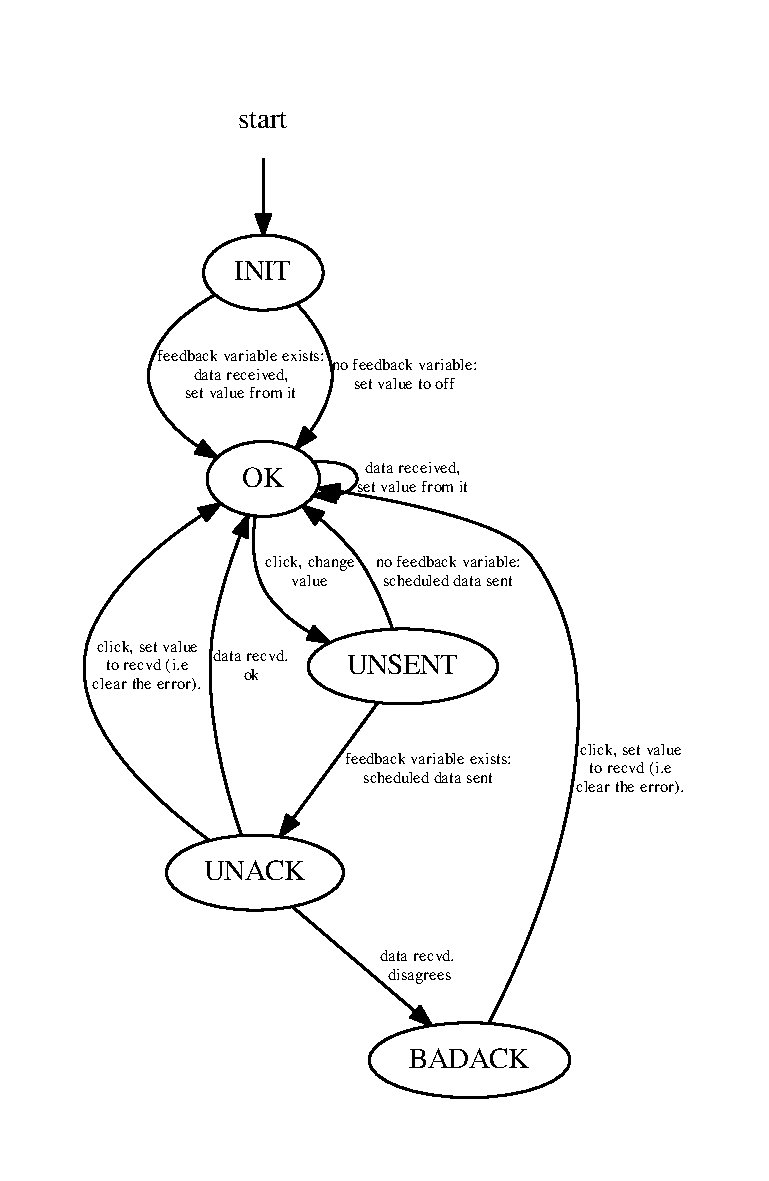
\includegraphics[width=4in]{stateSwitch.pdf}
\caption{State diagram for switches}
\label{switchstates}
\end{figure}
See Section~\ref{secclient} for details of how to write remote code to deal with switches,
or use the code in the \texttt{sampleClient} directory as a template.

Switch specifications consist of a position, the name of an
output variable to use in the send packets, a title,
an an optional feedback source. There may also be the word \verb+always+, in which case the value for this switch
is always sent, whenever any other output widget changes and when the send interval elapses; and the word \verb+immediate+ 
indicating that when the switch is pressed, a UDP send update should be done immediately. This will result in the
switch's data being sent, as well as any data for other `always' output widgets. The word \verb+button+ will make the switch
look more like a momentary button than a crude toggle. It's a purely visual change.

If \verb+integer+  is set, the switch will round all values it sends --- this is important if the value is converted to an integer
at the remote end, because otherwise the feedback value will not match the original float value of the slider.
\begin{v}
switch      ::= 'switch' pos '{'
                    'out' ident
                    ['button']
                    [ 'size' int ',' int]
                    [ 'title' string ]
                    [ source ]
                    [ 'set' float ]
                    [ 'always' ]
                    [ 'immediate' ]
                    [ 'integer' ]
                    [ 'key' keyname ]
                    [ 'colours' oncolour ',' offcolour ]
                '}'

oncolour    ::= colour
offcolour   ::= colour
\end{v}

\subsubsection{Multi-way switches with `set'}
It's often necessary to be able to set a control variable to multiple discrete values --- for example, an integer indicating an
operating mode. To support this, switches can have a `set' value which they send instead of the normal `toggle' operation. The differences
are:
\begin{itemize}
\item Instead of toggling the value between 0 and 1 and sending it when clicked, `set' switches always send their `set' value.
\item When feedback arrives on a set switch in the OK state, the switch value is set to off if the feedback does not match the set value,
and on if it does.
\item When feedback arrives on a set switch in the BADACK state, the switch is set to on if the feedback agrees, and BADACK if it doesn't (i.e.
the normal behaviour.)
\end{itemize}
We can therefore manage multiple values with a set of switches, all controlling the same control variable with different values. For example,
consider a three state system: OFF, HOLD and RUN. Let's assume that the integer values for these states are 0, 1 and 2 respectively; and that
the control and feedback telemetry variables are both called `runstate'. We can set up switches to control the state like this:
\begin{v}
    switch 0,0 { button out runstate var runstate set 0 title "OFF"}
    switch 1,0 { button out runstate var runstate set 1 title "HOLD"}
    switch 2,0 { button out runstate var runstate set 2 title "RUN"}
\end{v}
If we click HOLD, \texttt{runstate=1} is sent. Remotely, runstate will be set to 1 and feedback
sent back to the monitor. The OFF and RUN switches will both be set to off, because the feedback
does not agree with their set value; and the HOLD switch will be set to on, because it does.

\subsubsection{A note on keys}
Note that a switch can have a key mapped onto it. The key name is a string (delimited by quotes)
which is either an ASCII character, or one of the following:

\begin{center}
\begin{tabular}{llll}
home & end & pgup & pgdn \\
ins & del & up & down \\
left & right & \\
\end{tabular}
\end{center}


\subsubsection{Momentary}
\label{moms}
A momentary button is an output widget, similar to a switch. It also has a
feedback source, in a similar manner to a switch --- the button's feedback is
valid if it is above 0.5 and the packet setting it arrives after the button
was pressed. You can change the condition by using a boolean expression, of course.
To specify a feedback source, use the `var' clause, either with a variable name
or with an expression.

A momentary button sets its output variable to 1 by default, but that can be changed
by using a `set' clause.

Momentary buttons use a similar colour scheme to that of a switch:
\begin{itemize}
\item \textbf{light grey} (OK) means the button is ready;
\item \textbf{green} (WAIT) means the button has recently been pressed and acknowledged (if in feedback mode),
and will soon return to the ready state (this a purely cosmetic state;)
\item \textbf{dark grey} (UNSENT) means the button has been pressed, but data has not yet been sent. You can set \emph{immediate} to
make sure a value is sent immediately on change;
\item \textbf{diagonal crosshatch} (UNACK) means the press has been sent (indicated by the colour) but a feedback value has
not yet been received --- if this persists it can be cleared with a click;
\item \textbf{full crosshatch} (BADACK) means a value has been sent (indicated by the colour) and a feedback value has
been received, but the two do not match (i.e. the value read is less than 0.5.) In this state, the button can be reset by clicking
it again, but this will \emph{not result in another send.} It simply clears the error state.
\end{itemize}
If there is no feedback source, the button will go straight to OK once the
value is sent. The button can only be clicked in OK, UNACK and BADACK states: clicking in
OK will send the value, clicking in BADACK will, as stated above, clear the error.
The state diagram in figure~\ref{momstates} shows this more clearly.
\begin{figure}[ht]
\center
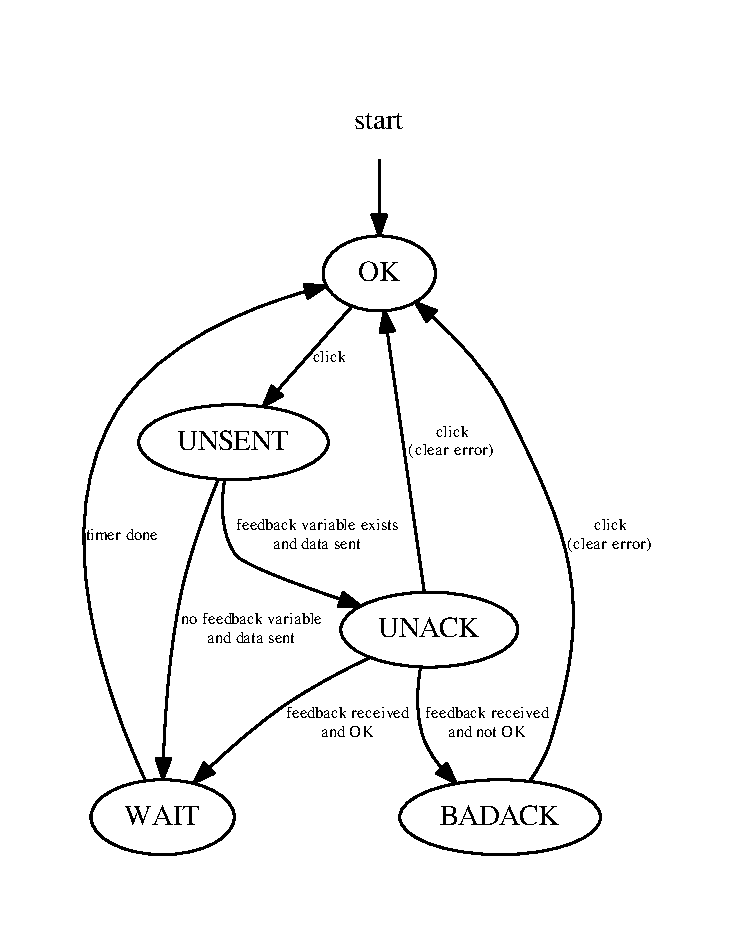
\includegraphics[width=4in]{stateMomentary.pdf}
\caption{State diagram for momentary buttons}
\label{momstates}
\end{figure}


See Section~\ref{secclient} for details of how to write remote
code to deal with momentary buttons.

Another use of momentary buttons is to `nudge' widgets controlling continuous
values, such as sliders. Instead of a \emph{out} clause with an output
variable name, the word \emph{nudge} and the name of the output variable of a
slider is used, along with an action: \emph{up,} \emph{down} and so on. A
feedback source is not permitted with nudge buttons.
\begin{v}
momentary  ::= 'momentary' pos '{'
                    ( 'out' ident |
                      'nudge' name ('up'|'down'|'centre'|'min'|'max') )
                    [ 'title' string ]
                    [ source ]
                    [ 'always' ]
                    [ 'set' float]
                    [ 'size' int ',' int]
                    [ 'immediate' ]
                    [ 'key' keyname ]
                    [ 'special' string ]
                '}'
\end{v}


\textbf{Special actions:} If the ``special'' string is given, the button will
perform a special action, hardwired into the code. Any other specified action,
such as an output to a variable or a nudge, will be ignored. The specials are
currently:
\begin{itemize}
\item \textbf{quit} will quit the program, sending the special string
\texttt{QUIT=1} over UDP as it does so.
\item \textbf{startlog} will start writing a log file of incoming UDP data
\item \textbf{stoplog} will start writing a log file
\item \textbf{resetmaps} will cause all maps to reset their bounding boxes to contain their items
\end{itemize}


\subsubsection{Slider}
Sliders are output widgets which control continuous values. They
work in a similar manner to switches, but the value controlled
is a floating point value over a specified range.

A feedback source can also be specified, which is compared against
the value which has been sent. The two values must be within
a user-configurable epsilon of each other for a match (currently 0.001).
To specify a feedback source, use the `var' clause, either with a variable name
or with an expression.

The handle of the slider shows:
\begin{itemize}
\item \textbf{dark yellow} (INIT) a feedback value exists but no value has yet been received
from the server to initialise the slider (one may have been sent if there is an `initial'
clause.)
\item \textbf{white} (OK) where the value matches the value on the server (or we
don't have a feedback source);
\item \textbf{grey} (UNSENT or DRAGGING) means data not yet sent or we're actively
dragging the slider, about to set a new value;
\item \textbf{diagonal crosshatch} (UNACK) means data sent but no acknowledgement;
\item \textbf{full crosshatch} (BADACK) means data sent, but the received value is not
yet within epsilon of the sent value. This is not necessarily an error,
it may take some time for the physical system to catch up.
\end{itemize}
In any state, the slider will move by itself as new data comes in with new values; also it's possible
to drag the slider to send a new value in any state (except INIT).

See ``Momentary'' for how to create button widgets which can nudge the slider.

It should be noted that \emph{immediate} with a slider works a little
differently from other widgets: the value will only be sent with the slider
handle is released. This is to avoid flooding the network with UDP packets as
the slider moves. However, using a autorepeat key on a key-mapped momentary
to nudge a slider which is set to immediate will result in many UDP packets
being sent!

\begin{v}
slider      ::= 'slider' pos '{'
                    'out' ident
                    'range' float 'to' float
                    'initial' float
                    'var' source
                    [ 'title' string ]
                    [ source ]
                    [ 'always' ]
                    [ 'immediate' ]
                    [ 'horizontal' | 'vertical' ]
                '}'
\end{v}
The state machine for the slider is shown in Figure~\ref{sliderstate}. Note how
almost any state will transition to DRAGGING if the slider is pressed --- this means
that many packets can be sent, even from UNACK and BADACK states.

\begin{figure}[ht]
\center
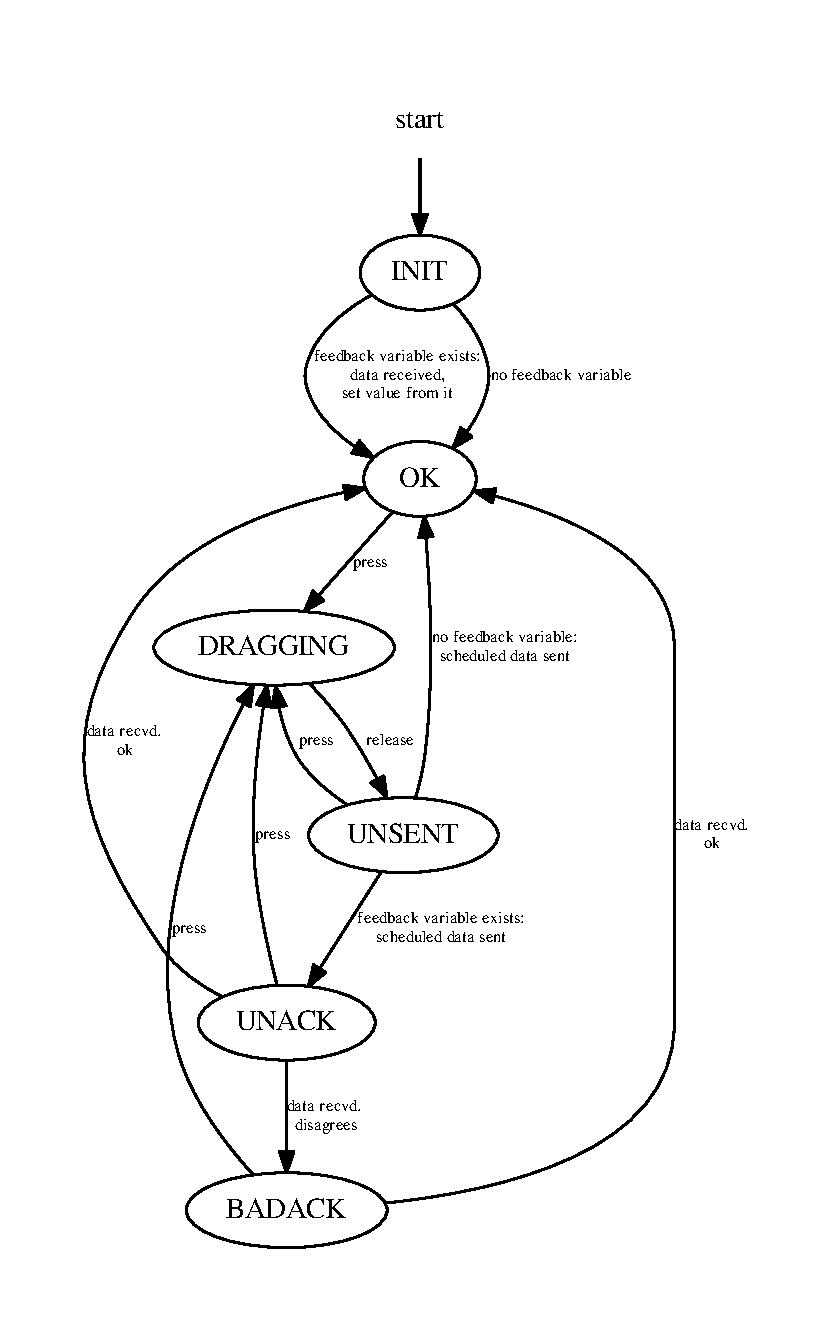
\includegraphics[width=4in]{stateSlider.pdf}
\caption{Slider state diagram}
\label{sliderstate}
\end{figure}

\section{Audio warnings}
These have the syntax:
\begin{v}
audio       ::= 'audio' source ( 'sample' | 'speech') string
\end{v}
They play either an audio sample or use text-to-speech to read a phrase whenever the source is above zero.
They will not trigger if an audio been played within the last two seconds. The checks are made every graphical
update tick --- by default two seconds, but changed with \texttt{updateinterval.} 

Typically, an expression source will be used. For example:
\begin{v}
    audio expr "a>0" range auto sample "warning.wav"
\end{v}
or 
\begin{v}
    audio expr "speed<5 && power>10" range auto speech "speed low and power high"
\end{v}
Audio warnings are currently implemented by using \verb+fork()+ and \verb+exec()+ 
to run \verb+/bin/espeak+ or \verb+/bin/aplay+. This is because audio APIs
in Qt are large and unwieldy, and often don't work.




\section{Other notes}

\subsection{How output data is sent}
\label{subhowout}
Whenever the output update runs, output data is sent for those widgets which
are either have changed since the last send, or are set to \emph{always send}.
The output update is run every \emph{sendinterval} seconds, which defaults to
2 seconds but can be set by the configuration file. In addition, widgets set
as \emph{immediate} cause the output update to run whenever they are changed.

Packets are sent to the same address the telemetry packets are coming from.


\subsection{Special variables}
Some variables are created at startup:
\begin{itemize}
\item \textbf{timesincepacket} is the number of seconds since the last packet
was received. It is updated every two seconds or so.
\item \textbf{lastpacketinterval} is the number of seconds between the last
packet and the packet before that. It is updated on every packet.
\end{itemize}

\section{Writing remotes}
\label{secclient}
\subsection{Telemetry}
The simple case is a telemetry-only remote, which just sends information to the monitor. This should send lines consisting
of a timestamp in seconds (preferably a UNIX timestamp) and variable values, all as floats in key=value pairs, terminated with
a line feed:
\begin{v}
time=1368451979.922781 a=33.326191 b=1.000000
time=1368451980.823072 a=33.339432
time=1368451981.723353 a=33.352539 b=2.000000
\end{v}
Only those variables which change at each tick need to be sent --- this is even true in the case of linked variables such as coordinate
pairs. Each line should be sent as a UDP packet --- currently we're using code like this:
\begin{v}
bool udpSend(const char *hostip, int port, const char *msg){
    sockaddr_in servaddr;
    int fd = socket(AF_INET,SOCK_DGRAM,0);
    if(fd<0){
        perror("cannot open socket");
        return false;
    }
    
    bzero(&servaddr,sizeof(servaddr));
    servaddr.sin_family = AF_INET;
    servaddr.sin_addr.s_addr = inet_addr(hostip);
    servaddr.sin_port = htons(port);
    if (sendto(fd, msg, strlen(msg)+1, 0, // +1 to include terminator
               (sockaddr*)&servaddr, sizeof(servaddr)) < 0){
        perror("cannot send message");
        close(fd);
        return false;
    }
    close(fd);
    return true;
}
\end{v}

\subsection{Control}
Controlling a remote system is a little more complex. We need to consider issues of latency and dropped packets carefully (see
the above sections on the slider, switch and momentary button to see how the controls work.) Data is sent from the monitor
to a UDP server on the remote, which optionally sends feedback information as part of the standard telemetry.

The control data packets are similar to the telemetry packets: a set of
key-value pairs, but no timestamp. They change a different set of values on
the remote from those monitored by telemetry. Control data is sent regularly
(if any values have changed) and can also be sent when immediate is set on a
control.

\subsubsection{Framework}
There is a framework for control data in the \texttt{sampleClient} directory, in \texttt{udpserver.h/.cpp}. This defines
a \texttt{UDPServer} class which can be used to create control variables, get values from them, and periodically poll for changes.

There are three kinds of control:
\begin{itemize}
\item toggle switch --- controls a 0/1 value which is toggled and resent each time the switch is flipped;
\item momentary button --- the same value (the ``set'' value, 1 by default) is sent as the value of the control variable every time the button is pressed;
\item slider --- controls a continuously varying floating point value, sent every time the slider is moved.
\end{itemize}

\subsubsection{Feedback}
It's a good idea to use a telemetry variable to shadow the control variables, sending any changes to the control variables
back to the monitor. This can be a variable of the same name, or a different name. It's also possible to use an expression as a feedback
value in the monitor.

\subsubsection{An example using UDPServer}
See \texttt{sampleClient/test.cpp} for a full example.

\include{waypoint}

\end{document}
